\documentclass[12pt]{article}
\usepackage[utf8]{inputenc}
\usepackage[spanish]{babel}
\usepackage{graphicx}
\usepackage{wrapfig}
\usepackage{amsmath}
\usepackage{amsfonts}
\usepackage{amssymb}
\usepackage[dvipsnames]{xcolor}
\title{Preparando Documentos Científicos con LATEX}
\author{Olga María Fimbres Morales}
\date{22 de Enero 2016}


\begin{document}
\maketitle
\pagebreak

Como nos dice \cite{Wik} "Las matemáticas de un péndulo son, en general, muy complicadas. Asumir simplificaciones, en el caso de un péndulo simple. nos permite resolver las ecuaciones analíticamente para oscilaciones de ángulos pequeños."
\section{Péndulo Simple.}


Un péndulo simple es una idalización de un péndulo real para le cual se  asumen las siguientes condiciones:\\
\begin{wrapfigure}{r}{6cm}
	\begin{center}
      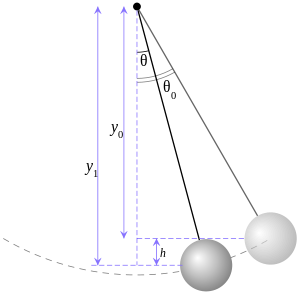
\includegraphics[width=6.0cm]{pendulo.png}
      \caption{Péndulo simple \cite{Img1}.}
    \end{center}
\end{wrapfigure}
\begin{itemize}
\item El cordón al cual se sujeta el peso posee una masa despreciable, además de ser rígido.
\item El peso se considera una masa puntual.
\item El movimiento solo ocurre en dos dimensiones, por lo que el peso no traza una elipse, si no un arco.
\item El péndulo no pierde energía ya que no se considera la fricción con el aire.
\item El campo gravitacional es uniforme.
\item El soporte no se mueve.
\end{itemize}

La ecuación diferencial que representa el movimiento de un péndulo simple es:
\begin{equation}
\textcolor{Red}{\frac{d^2 \theta}{dt^2} + \frac{g}{l}\sin\theta = 0}
\end{equation}

donde $g$ es la aceleración de la gravedad, $l$ es la longitud del péndulo y $\theta$ es el ángulo de desplazamiento.

\pagebreak
\section{Aproximaciones para ángulos pequeños.}

La ecuación diferencial que describe el movimiento del péndulo simple no resulta fácil de resolver, además de que las soluciones no pueden ser escritas en términos de funciones elementales. Aún así si se le restringe el valor para el ángulo de oscilación, la ecuación puede resolverse de una forma sencilla. Si se asume que el ángulo sera mucho más pequeño que 1 radian o $\theta \ll 1 $, con un error de orden de $\theta ^3$, se obtiene lo siguiente:
\begin{eqnarray*}
\sin \theta \approx \theta \\
\frac{d^2 \theta}{dt^2} + \frac{g}{l}\theta = 0
\end{eqnarray*}

Tomando como condiciones iniciales $\theta (0) = \theta_0$ y $d\theta l dt(0) = 0$, la solución resulta en:
\begin{eqnarray*}
\theta(t) = \theta_0 \cos \left( \sqrt{\frac{g}{l}t} \right)  \qquad \theta_0 \ll 1 
\end{eqnarray*}

El movimiento es un movimiento armónico simple donde $\theta_0$ es la semi-amplitud de oscilación. El periodo de oscilación es:
\begin{eqnarray*}
T_0 = 2\pi \sqrt{\frac{l}{g}}  \qquad   \qquad  \theta_0 \ll 1
\end{eqnarray*}
lo cual se conoce como la ley de Christiaan Huygens para el periodo; nótese que para pequeños ángulos el periodo resulta independiente de la amplitud $\theta_0$.


\pagebreak
\section{Amplitudes Arbitrarias.}

Cuando se trabaja con amplitudes más grandes, es posible, por medio de un programa computacional, calcular el periodo exacto invirtiendo la ecuación de la velocidad angular obtenida por medio de la energía:
\begin{wrapfigure}{r}{7cm}
	\begin{center}
      \includegraphics[width=7.0cm]{pendulo2.png}
      \caption{Desviación del periodo\cite{Img2}.}
    \end{center}
\end{wrapfigure}
\begin{equation}
\textcolor{Red}{\frac{dt}{d \theta} = \sqrt{\frac{l}{2g}} \frac{1}{\sqrt{\cos\theta -  \cos\theta_0}}}
\end{equation}

y después integrando sobre un ciclo completo
\begin{eqnarray*}
T = t(\theta_0 \to 0 \to -\theta_0 \to 0 \to \theta_0)
\end{eqnarray*}

o dos veces un medio ciclo
\begin{eqnarray*}
T=2t(\theta_0 \to 0 \to -\theta_0)
\end{eqnarray*}

o cuatro veces un cuarto de ciclo
\begin{eqnarray*}
T=4t(\theta_0 \to 0)
\end{eqnarray*}

lo cual nos lleva a
\begin{eqnarray*}
T=4 \sqrt{\frac{l}{2g}}\int\limits_0^{\theta_0} \frac{1}{\sqrt{\cos\theta - \cos\theta_0}} d\theta
\end{eqnarray*}

Esta integral puede ser reescrita en términos de una integral elíptica como
\begin{eqnarray*}
T=4 \sqrt{\frac{l}{2g}}F\left( \frac{\theta_0}{2}, \csc\frac{\theta_0}{2} \right)
\end{eqnarray*}

donde $F$ es es la integral elíptica incompleta de primer tipo, definida como:
\begin{eqnarray*}
F(\rho, k) = \int\limits_0^{\rho} \frac{1}{\sqrt{1 -(k^2)\sin^2 u}}du
\end{eqnarray*}

O mas concisamente utilizando la sustitución $\sin u = \frac{\sin\frac{\theta}{2}}{\sin\frac{\theta_0}{2}}$ expresando $\theta$ en términos de $u$,
\begin{equation}
\textcolor{Red}{T=4\sqrt{\frac{l}{g}}K\left( \sin^2 \left(\frac{\theta_0}{2} \right) \right)}
\end{equation}

donde $k$ es la integral elíptica completa de primer tipo, definida por
\begin{eqnarray*}
K(k) = F \left( \frac{\pi}{2}, k \right) = \int\limits_0^{\frac{\pi}{2}} \frac{1}{\sqrt{1-k^2 \sin^2 u}}du
\end{eqnarray*}

Comparando la aproximación con la solución completa, considerando el periodo de un péndulo de un metro de longitud en la Tierra a un ángulo inicial de 10 grados $T \approx 2.0102 s$. La aproximación lineal es $T \approx 2.0064 s$. La diferencia entre estos dos valores es de menos del 0.02\%, lo cual resulta mucho menor que la variación causada por la gravedad dependiendo de la localización geográfica. Es por eso que existen muchas maneras de calcular la integral elíptica:

\subsection{Solución del polinomio de Legendre para la integral elíptica}

Utilizando la ecuación (3) y el polinomio de Legendre para la solucieqnarrayón de la integral elíptica:
$$K(k) = \frac{\pi}{2} \left\{ 1 + \left( \frac{1}{2} \right) ^2 k^2 + \left( \frac{1 * 3}{2*4} \right)^2 k^4 + ... + \left[\frac{(2n-1)!!}{(2n)!!} \right] ^2 k^{2n} + ... \right \}$$


Donde $n!!$ denota un doble factorial, una solución exacta para el periodo del péndulo es:

$$T=2\pi \sqrt{\frac{l}{g}} \left( 1 + \left( \frac{1}{2} \right) ^2 
									\sin^2 \left( \frac{\theta_0}{2} \right)
									 + \left( \frac{1*3}{2*4} \right)^2 
									 \sin^4 \left( \frac{\theta_0}{2} \right) 
									 + \left( \frac{1*3*5}{2*4*6} \right)^2 
									 \sin^6 \left( \frac{\theta_0}{2} \right) \right) $$\\
$$= 2\pi \sqrt{\frac{l}{g}} \sum_{n=0}^\infty \left[ \left( \frac{(2n)!}{(2^n * n!)^2} \right)^2 \sin^{2n} \left( \frac{\theta_0}{2} \right) \right]
$$

La gráfica nos muestra los errores relativos utilizando la serie de potencias. $T_0$ es la aproximación lineal, y $T_2$ a $T_10$ incluyen, respectivamente, la segunda y décima potencia.

\subsection{Solución de serie de potencias para la integral elíptica}
\begin{wrapfigure}{l}{5.5cm}
	\begin{center}
      \includegraphics[width=5.5cm]{pendulo3.png}
      \caption{Errores relativos utilizando serie de potencias\cite{Img3}.}
    \end{center}
\end{wrapfigure}
\\
Otra formulación de la solución anterior puede ser encontrada si se sigue la serie de Maclaurin:
$$
\sin\frac{\theta_0}{2} = \frac{1}{2}\theta_0 - \frac{1}{48}\theta_{0}^{3} + \frac{1}{3840}\theta_{0}^{5} - \frac{1}{645120}\theta_{0}^{7}+...
$$
\\
\\
es utilizada en la solución del polinomio de Legendre. Las potencias resultantes son:
\begin{eqnarray*}
T= 2\pi \sqrt{\frac{l}{g}} \left( 1 + \frac{1}{16}\theta_{0}^{2} + \frac{11}{3072}\theta_{0}^{4} + \frac{173}{737280}\theta_{0}^{6} +\\ \frac{22931}{1321205760}\theta_{0}^{8}+ \frac{1319183}{951268147200}\theta_{0}^{10} + ...\right)
\end{eqnarray*}
\\

\subsection{Solución media aritmética-geométrica para la integral elíptica}

Utilizando la ecuación (3) y la solución media aritmética-geométrica:
$$
K(k)= \frac{\pi / 2}{M(1-k,1-k)}
$$
donde $M(x,y)$ es el significado aritmétrico-geométrico de $x$ y $y$. Esto nos proporciona una fórmula alternativa más rápida para el periodo:

\begin{eqnarray*}
T=\frac{2\pi}{M(1,\cos(\theta_0 /2))}\sqrt{\frac{l}{g}}
\end{eqnarray*}

\pagebreak
\begin{thebibliography}{X}
 \bibitem{Wik} \textsc{Wikipedia, The free encyclopedia; "Pendulum (mathematics)"; 2016}
 \bibitem{Img1} \textsc{By Krishnavedala; via Wikimedia Commons;"Pendulum (mathematics)"}
 \bibitem{Img2} \textsc{By Alessio Damato; via Wikimedia Commons;"Pendulum (mathematics)"}
 \bibitem{Img3} \textsc{By Rui Ferreira; via Wikimedia Commons;"Pendulum (mathematics)"}
\end{thebibliography}

\end{document}
